\chapter{Fundamentação Teórica}

\lipsum[43-45]

\section{Aprendizado de Máquina e \textit{Deep Learning}}
\lipsum[45]
% TODO Pensar em como introduzir conceitos mais usados nas soluções STR, como deconv, fully convolutional, skip copnnections
\subsection{Linguagens de Programação e \textit{Frameworks}}
\lipsum[45]

\section{Evolução do \textit{Scene Text Recognition}}
\lipsum[45]
\subsection{Detecção de Texto}
\lipsum[25]

\subsubsection{CRAFT}\label{craft}
Character Region Awareness for Text Detection \cite{CRAFT}, ou simplesmente CRAFT, é um método de detecção publicado por Youngmin Baek et al. (2019), integrantes do time de pesquisa da empresa coreana Naver Corporation\cite{NaverCorp}, que apresentou resultados bastante competitivos quando comparado aos resultados estado-da-arte do momento, superando as melhores soluções do momento em acurácia de detecção com desempenho, capacidade de detecção em frames por segundo, competitiva com os melhores métodos já publicados.
	
Youngmin Baek et al. introduz um método de detecção a nível de caractere onde um modelo de rede convolucional FCN é criado a partir da reconhecida rede de extração de feature VGG-16\cite{VGG}. A arquitetura da rede CRAFT se inspirou na rede U-Net \cite{UNET} ao introduzir skip-connections, agregando características de alto e baixo nível entre os blocos de upsampling, que decodificam o mapa de predição em dois resultados ao final da rede:

\begin{itemize}
    \item {Mapa de predição de região de carácter (\textit{Character Region Score}): probabilidades de cada pixel está localizado no centro de um carácter}
    \item {Mapa de predição de afinidade entre caracteres (\textit{Character Afiinity Score}): Probabilidades de cada  pixel está localizado no centro da região entre caracteres}
\end{itemize}

Como o resultado da rede é bem específico, as imagens de \textit{ground truth} são geradas a partir de processamento de imagens. A partir das \textit{bounding boxes} de cada caractere, um \textit{heatmap} de uma distribuição gaussiana é projetada dentro de cada região de caractere, representando uma distribuição de probabilidade onde o centro da distribuição é o centro da região de caractere. Com isso tem-se o gabarito do primeiro resultado da rede. O \textit{ground truth} para as regiões de afinidade envolve novamente projetar um heatmap gaussiano em uma região que, agora, é calculada em tempo de execução a partir dos \textit{bounding boxes} de cada caractere. A Fig. \ref{fig:craft_gt}  ilustra o método utilizado, que se baseia em calcular uma região retangular entre caracteres utilizando os centroides dos caracteres vizinhos e centroides de triângulos gerados em cada caractere.

\begin{figure}
    \centering
    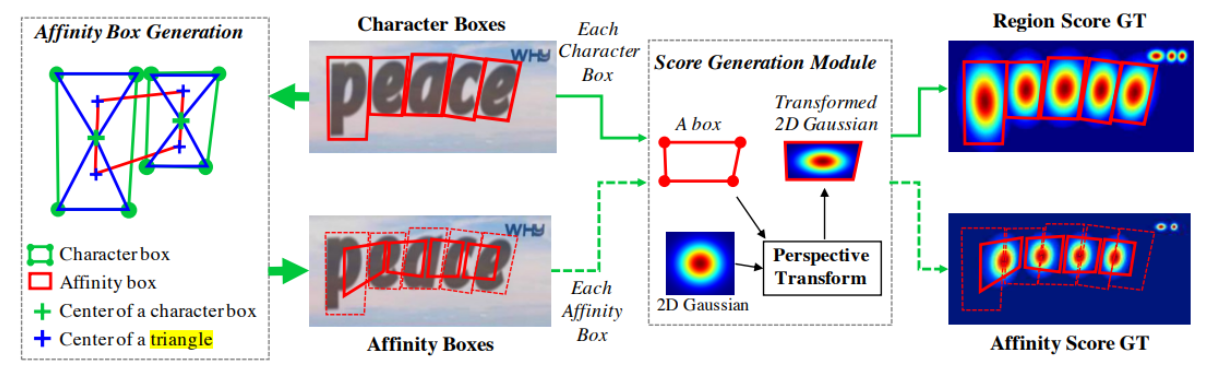
\includegraphics[width=\textwidth]{figs/craft-gt.png}
    \caption{Ilustração das etapas de geração dos arquivos de ground truth para a etapa de treino do CRAFT. Fonte [\citeonline{CRAFT}]}
    \label{fig:craft_gt}
\end{figure}

Para treinar a rede, os autores se utilizaram de uma estratégia de aprendizado levemente supervisionado. Como as principais bases de imagens para treinamento não contam com anotações a nível de caracteres, a rede primariamente é treinada com imagens com texto sintético, usando o dataset SynthText \cite{SynthText}.

Para refinar o treino em datasets com imagens de cenas reais, os autores utilizam a própria rede treinada em texto sintético para predizer as regiões de caracteres das imagens de cena para gerar anotações a nível de caracteres para as imagens dos datasets utilizados com auxílio de métodos de processamento de imagem, conforme exemplificado na Fig. \ref{fig:craft_char_level_annotation}. O processo contém as seguintes etapas:

\begin{itemize}
    \item \textit{Cropping}: Extração das palavras que possuem região descrita nos arquivos de \textit{ground truth} dos datasets de benchmark.
    \item \textit{Character Split}: Processo de localização e segregação de cada caractere detectado pela rede treinada em base de dados sintética. A rede a partir das imagens provenientes da etapa de \textit{Cropping}, predizendo as regiões onde a probabilidade de existir um caractere. Com a localização dessas regiões, é aplicado o algoritmo de segmentação conhecido como Watershed \cite{WatershedOverview}, cujo objetivo é expandir a área de um caractere a partir do centro da região de maior probabilidade até que as áreas de caracteres adjacentes se encontrem. Isso faz com que seja possível ajustar um bounding-box em volta de cada caractere observado.
    \item \textit{Unwarping}: Uma vez em posse da capacidade de localizar todos os caracteres, obtida através da etapa de \textit{Character Split}, pode-se projetar as coordenadas para as \textit{bounding-boxes} de cada caractere de volta para a imagem original aplicando as operações inversas às aplicadas na etapa de \textit{Cropping}
\end{itemize}

Com essas labels geradas sobre as imagens reais dos datasets de benchmark, os gabaritos para o treinamento do modelo completo são gerados conforme explicado anteriormente e o treinamento da rede é refinado com esses novos exemplos.

\begin{figure}
    \centering
    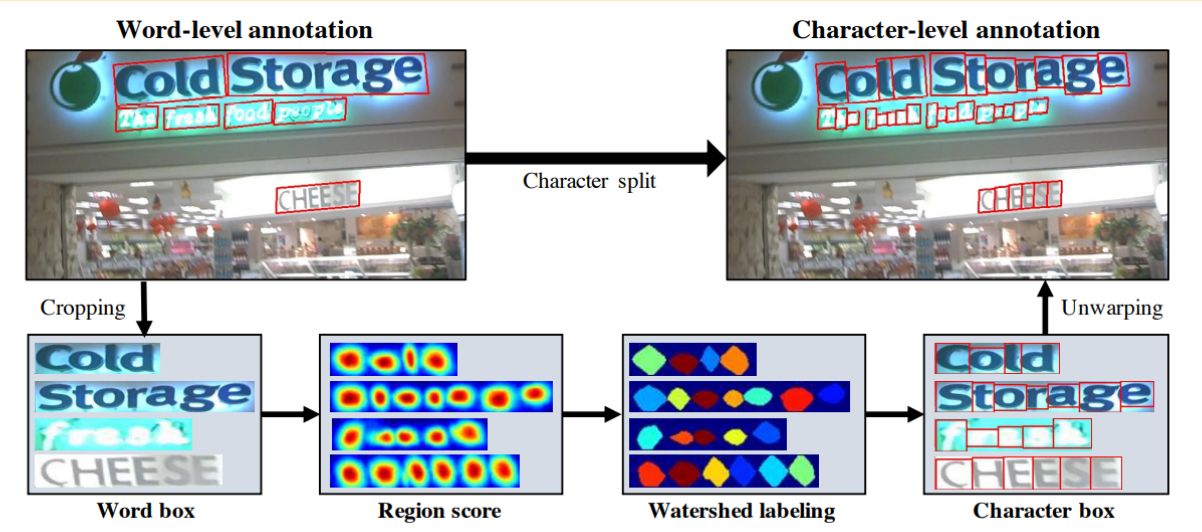
\includegraphics[width=\textwidth]{figs/craft-char-level-annotation.png}
    \caption{Exemplificação do passo a passo para geração de anotações a nível de caracteres durante a etapa de treino do CRAFT. Fonte [\citeonline{CRAFT}].}
    \label{fig:craft_char_level_annotation}
\end{figure}

O CRAFT conta com um pós-processamento bastante simplificado em cima dos mapas de probabilidade que são gerados pela rede com o intuito de calcular os bounding boxes do texto localizado, que envolve, novamente com auxílio de métodos de visão computacional e processamento de imagem. Usando binarização e categorização, é possível unir as regiões de caracteres e de afinidade para extrair as coordenadas dos menores retângulos que encapsulam o resultado dessa união.

\subsection{Reconhecimento de Texto}
\lipsum[25]


\subsubsection{CRNN} \label{crnn}
% TODO Elaborar um pouco mais o CRNN
Convolutional Recurrent Neural Networks \cite{CRNN}, introduzido por Baoguang Shi et al. é uma solução para o problema de reconhecimento de texto bastante popular, sendo bastante citada em novos trabalhos e sempre presente em trabalhos comparativos. Este método veio para resolver grandes dificuldade das soluções anteriores, por exemplo: lidar com entradas e saídas de comprimentos variados, possibilitar o aprendizado conhecido como end-to-end, isto é, aplicar uma função de perda sobre o resultado do reconhecimento e essa perda ser propaganda para o aprendizado da rede extratora de características.

O CRNN, como o nome sugere, une uma rede neural convolucional, sem as camadas de predição totalmente conectadas, para gerar os feature maps sobre a imagem de entrada. Esses mapas são sequenciados para que alimentem a rede neural recorrente (RNN), que é responsável por conseguir decodificar cada sequência em um possível caractere. A Fig. \ref{fig:crnn_pipeline} ilustra o pipeline de processamento que essa arquitetura executa.

\begin{figure}
    \centering
    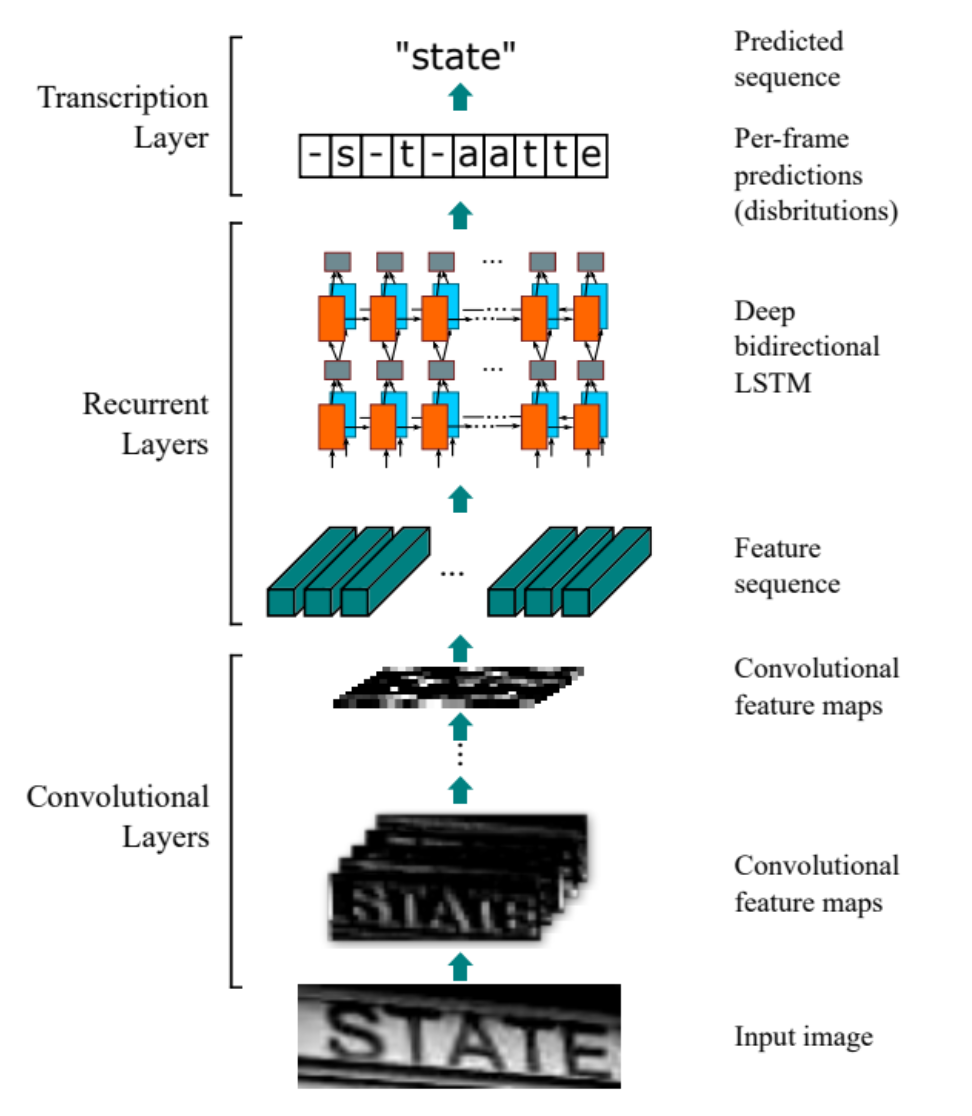
\includegraphics[width=0.75\textwidth]{figs/crnn-pipeline.png}
    \caption{Ilustração do pipeline de reconhecimento do CRNN. Fonte [\citeonline{CRNN}].}
    \label{fig:crnn_pipeline}
\end{figure}

A rede RNN que é implementada no CRNN faz uso de atributos LSTM (\textit{Long-Short Term Memory}) bi-direcional, pois por estar visando reconhecimento de texto em cenas, muitas vezes carregar o contexto de sequências passadas e futuras é importante para diferenciar caracteres ou possibilitar o reconhecimento de um caractere, por exemplo, uma letra um pouco mais larga.

Os resultados obtidos foram bastante competitivos quando comparados aos métodos de reconhecimento anteriores, até mesmo superiores aos que já faziam uso dos conceitos de deep learning, com o adicional de prover meios de aprendizado integrado da rede convolucional e recorrente como uma unidade, além de um modelo bem mais enxuto em número de parâmetros\cite{CRNN}.

Por lidar com o reconhecimento como um problema de sequência, o modelo pressupõe que a orientação do texto é necessariamente da esquerda para a direita, isso leva a uma limitação, que seria reconhecer textos com não exatamente horizontais e retilíneos.


\section{Considerações Finais}

\lipsum[23]
